\begin{figure}[H]
	\begin{subfigure}{0.5\textwidth}
		\centering
		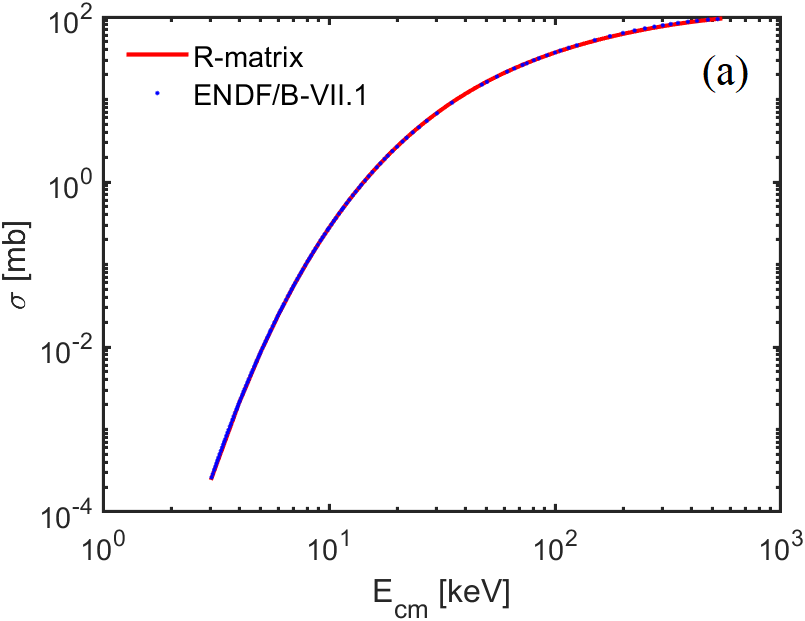
\includegraphics[width=1\textwidth]{image/chap03/section_compare_ddn.png}
	\end{subfigure}
	\begin{subfigure}{0.5\textwidth}
		\centering
		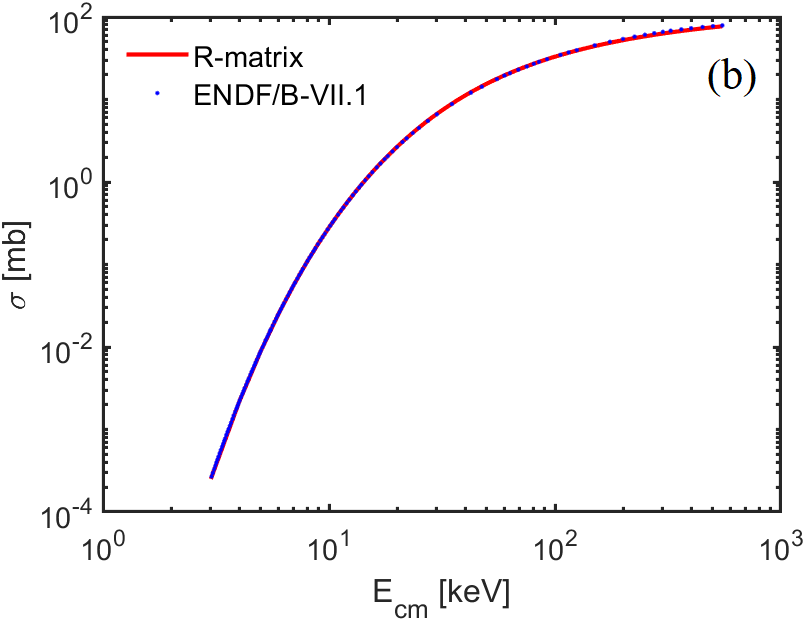
\includegraphics[width=1\textwidth]{image/chap03/section_compare_ddtp.png}
	\end{subfigure}
	\\
	\begin{subfigure}{1\textwidth}
		\centering
		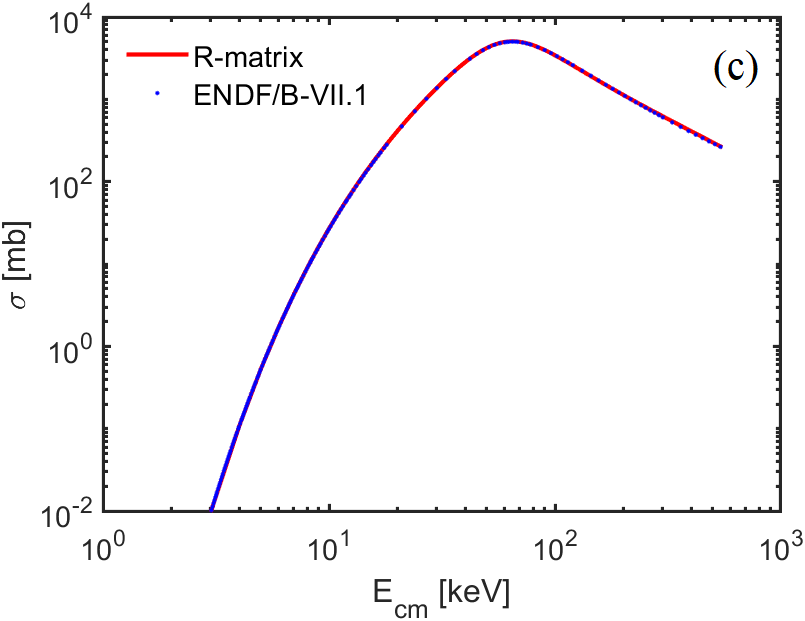
\includegraphics[width=0.5\textwidth]{image/chap03/section_compare_dt.png}
	\end{subfigure}
	\caption{R-matrix理论与ENDF/B-VII.1数据库对比。\\ (a) D(d, n)$^{\text{3}}$He;(b) D(d, p)T;(c) T(d, n)$ ^{\text{4}} $He}
	\label{fig:section_compare}
\end{figure}